% ------------------------------------------------------------------------------
% TYPO3 Version 10.3 - What's New (Italian Version)
%
% @license	Creative Commons BY-NC-SA 3.0
% @link		https://typo3.org/help/documentation/whats-new/
% @language	Italian
% ------------------------------------------------------------------------------

\section{Modifiche per integratori}
\begin{frame}[fragile]
	\frametitle{Modifiche per integratori}

	\begin{center}\huge{Capitolo 2:}\end{center}
	\begin{center}\huge{\color{typo3darkgrey}\textbf{Modifiche per integratori}}\end{center}

\end{frame}

% ------------------------------------------------------------------------------
% Feature | 90333 | Dashboard

\begin{frame}[fragile]
	\frametitle{Modifiche per integratori}
	\framesubtitle{Dashboard}

	% decrease font size for code listing
	\lstset{basicstyle=\tiny\ttfamily}

	\begin{itemize}
		\item I \textit{preset} della dashboard possono essere configurati per i nuovi utenti o
		    per gli utenti che hanno eliminato tutte le loro dashboard.
		\item Questo può essere utilizzato per mostrare una dashboard "Guida introduttiva" come impostazione predefinita.
		\item Esempio di TSconfig:

\vspace{-0.4cm}
\begin{lstlisting}
options.dashboard.dashboardPresetsForNewUsers = default, dashboardPreset-myPreset
\end{lstlisting}

		\item È possibile definire più preset della dashboard in un elenco separato da virgole.

	\end{itemize}

\end{frame}

% ------------------------------------------------------------------------------
% Important | 89992 | Use New TranslationServer

\begin{frame}[fragile]
	\frametitle{Modifiche per integratori}
	\framesubtitle{Piattaforma di gestione traduzione}

	\begin{itemize}
		\item La soluzione SaaS "\href{https://crowdin.com/}{Crowdin}" è ora utilizzata come piattaforma
			di gestione delle localizzazioni/traduzioni di TYPO3.
		\item Incoraggiamo tutti a partecipare e migliorare la localizzazione.
		\item Crowdin può essere utilizzato per tradurre le stringhe del core di TYPO3
			e delle estensioni di TYPO3.
		\item Leggi di più riguardo questo nella
			\href{https://docs.typo3.org/m/typo3/reference-coreapi/master/en-us/ApiOverview/Internationalization/TranslationServer/Crowdin.html}{documentazione TYPO3}.
	\end{itemize}

	\begin{figure}
		
\includegraphics[width=0.40\linewidth]{ChangesForIntegrators/crowdin-logo.png}
	\end{figure}

\end{frame}

% ------------------------------------------------------------------------------
% Feature | 90266 | Fluid-based templated emails

\begin{frame}[fragile]
	\frametitle{Modifiche per integratori}
	\framesubtitle{Email HTML basate su Fluid (1)}

	% decrease font size for code listing
	\lstset{basicstyle=\smaller\ttfamily}

	\begin{itemize}
		\item TYPO3 ora supporta l'invio di e-mail HTML e di testo basate su template.
		\item Le e-mail vengono create utilizzando il motore di template Fluid.
		\item I template delle e-mail possono essere personalizzati sovrascrivendo i percorsi dei file di template:

\vspace{-0.4cm}
\begin{lstlisting}
$GLOBALS['TYPO3_CONF_VARS']['MAIL']['templateRootPaths'][700] =
  'EXT:my_site_extension/Resources/Private/Templates/Email';

$GLOBALS['TYPO3_CONF_VARS']['MAIL']['layoutRootPaths'][700] =
  'EXT:my_site_extension/Resources/Private/Layouts';
\end{lstlisting}

	\end{itemize}

\end{frame}

% ------------------------------------------------------------------------------
% Feature | 90266 | Fluid-based templated emails

\begin{frame}[fragile]
	\frametitle{Modifiche per integratori}
	\framesubtitle{Email HTML basate su Fluid (2)}

	\begin{itemize}
		\item Le e-mail basate su template Fluid vengono utilizzate, ad esempio, per i seguenti componenti:

			\begin{itemize}
				\item Test email dell'Install Tool (vedi l'esempio nella slide seguente).
				\item Email di notifica dello workspace sul cambio di stage.
				\item Email di notifica sull'accesso utente di backend.
			\end{itemize}

	\end{itemize}

\end{frame}

% ------------------------------------------------------------------------------
% Feature | 90266 | Fluid-based templated emails

\begin{frame}[fragile]
	\frametitle{Modifiche per integratori}
	\framesubtitle{Email HTML basate su Fluid (3)}

	Email di test inviata dall'Install Tool:

	\begin{figure}
		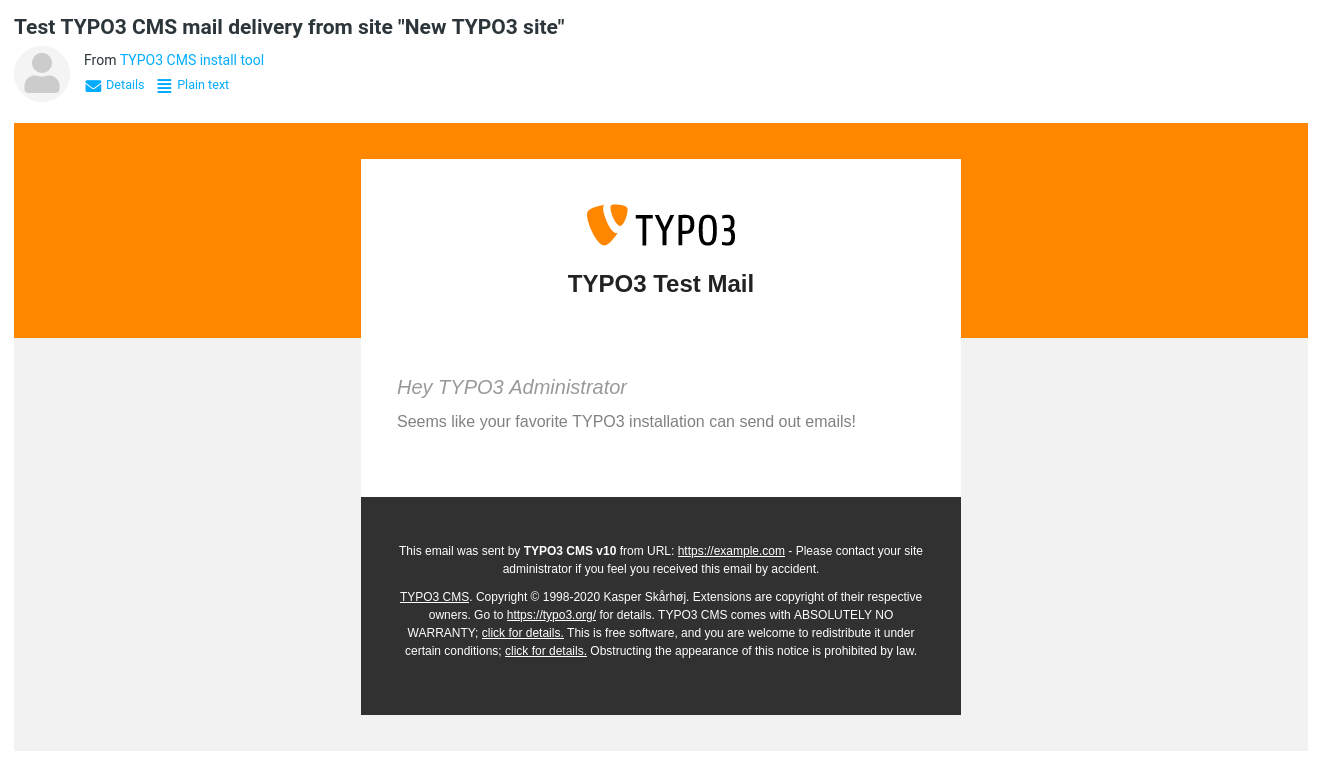
\includegraphics[width=0.8\linewidth]{ChangesForIntegrators/90266-FluidBasedTemplatedEmails.png}
	\end{figure}

\end{frame}

% ------------------------------------------------------------------------------
% Feature | 90203 | Make workspace available in TypoScript conditions

\begin{frame}[fragile]
	\frametitle{Modifiche per integratori}
	\framesubtitle{Workspace e TypoScript}

	% decrease font size for code listing
	\lstset{basicstyle=\smaller\ttfamily}

	\begin{itemize}
		\item È stata aggiunta una nuova variabile del linguaggio delle condizioni: \texttt{workspace}.
		\item Questa variabile può essere utilizzata per abbinare una determinata espressione a parametri comuni dello workspace.
		\item Attualmente sono supportati i seguenti parametri:\newline
			\small
				\texttt{workspaceId}, \texttt{isLive}, e \texttt{isOffline}.
			\normalsize
		\item Per esempio:

\vspace{-0.4cm}
\begin{lstlisting}
[workspace.workspaceId === 3]
  # Current workspace ID is 3
[end]
\end{lstlisting}

	\end{itemize}

\end{frame}

% ------------------------------------------------------------------------------
% Feature | 88962 | Re-implement old PIDupinRootline TypoScript condition

\begin{frame}[fragile]
	\frametitle{Modifiche per integratori}
	\framesubtitle{TypoScript}

	% decrease font size for code listing
	\lstset{basicstyle=\smaller\ttfamily}

	\begin{itemize}
		\item La vecchia condizione \texttt{PIDupinRootline} è stata reimplementata
			in TypoScript utilizzando il linguaggio delle espressioni di Symfony.
		\item Sintassi della vecchia condizione TypoScript:

\vspace{-0.4cm}
\begin{lstlisting}
[PIDupinRootline = 30]
  page.10.value = Sono su qualsiasi sottopagina della pagina con UID 30.
[END]
\end{lstlisting}

		\item Nuova sintassi di condizione TypoScript:

\vspace{-0.4cm}
\begin{lstlisting}
[30 in tree.rootLineParentIds]
  page.10.value = Sono su qualsiasi sottopagina della pagina con UID 30.
[END]
\end{lstlisting}

	\end{itemize}

\end{frame}

% ------------------------------------------------------------------------------
% Feature | 90426 | Browser-native lazy loading for images

\begin{frame}[fragile]
	\frametitle{Modifiche per integratori}
	\framesubtitle{Caricamento Lazy per le immagini}

	% decrease font size for code listing
	\lstset{basicstyle=\smaller\ttfamily}

	\begin{itemize}
		\item L'attributo HTML \texttt{loading} può essere impostato per i tag \texttt{<img>}.
		\item I browser che supportano questa funzione non caricheranno queste immagini finché non saranno nella finestra.
		\item Il comportamento può essere modificato dalla seguente costante TypoScript:

\vspace{-0.4cm}
\begin{lstlisting}
styles.content.image.lazyLoading = lazy
\end{lstlisting}

		\item Valori validi sono: \texttt{lazy} (default), \texttt{eager}, e \texttt{auto}.
		\item il ViewHelper Fluid \textit{Image} supporta anch'esso il caricamento lazy:

\vspace{-0.4cm}
\begin{lstlisting}
<f:image src="{fileObject}" treatIdAsReference="true"
  loading="lazy" />
\end{lstlisting}

	\end{itemize}

\end{frame}

% ------------------------------------------------------------------------------
% Important | 89869 | Change lockIP default to disabled for both frontend and backend

\begin{frame}[fragile]
	\frametitle{Modifiche per integratori}
	\framesubtitle{Valori preimpostati per \texttt{lockIP}/\texttt{lockIPv6}}

	% decrease font size for code listing
	\lstset{basicstyle=\smaller\ttfamily}

	\begin{itemize}
		\item Il valore di default per l'impostazione \texttt{lockIP} è stato modificato.
		\item Le seguenti quattro variabili di sistema sono \textbf{disabilitate} di default:

			\begin{itemize}
				\item \texttt{[FE]['lockIP']}
				\item \texttt{[FE]['lockIPv6']}
				\item \texttt{[BE]['lockIP']}
				\item \texttt{[BE]['lockIPv6']}
			\end{itemize}

		\item I vecchi valori preimpostati ("\texttt{4}" per il backend e "\texttt{2}" per il frontend)
			causavano problemi, ad esempio per i client con supporto degli indirizzi IPv4 e IPv6.

	\end{itemize}

\end{frame}

% ------------------------------------------------------------------------------
% Feature | 90052 | Form YAML configuration available in configuration module

\begin{frame}[fragile]
	\frametitle{Modifiche per integratori}
	\framesubtitle{Form: Configurazione YAML}

	\begin{columns}[T]
		\begin{column}{.04\textwidth}
		\end{column}
		\begin{column}{.38\textwidth}

			Se l'estensione di sistema \texttt{EXT:form} è installata, la configurazione YAML caricata
			può essere visualizzata in \textbf{SYSTEM} $\rightarrow$ \textbf{Configuration}.

			\vspace{0.2cm}

			Ciò richiede anche l'attivazione da parte degli amministratori di \texttt{EXT:lowlevel} naturalmente.

		\end{column}
		\begin{column}{.58\textwidth}
			\vspace{-0.3cm}
			\begin{figure}
				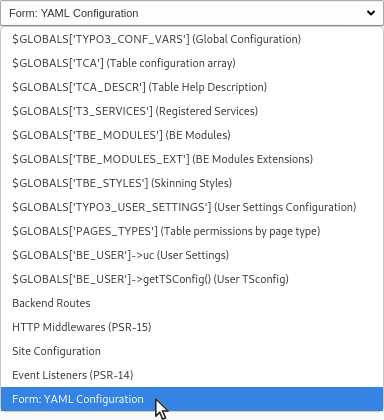
\includegraphics[width=0.70\linewidth]{ChangesForIntegrators/90052-AddYamlConfigurationToConfigurationModule.png}
			\end{figure}
		\end{column}
	\end{columns}

\end{frame}

% ------------------------------------------------------------------------------
% Feature | 88147 | Add possibility to configure the path to sitemap xslFile

\begin{frame}[fragile]
	\frametitle{Modifiche per integratori}
	\framesubtitle{SEO: \texttt{Sitemap.xsl}}

	% decrease font size for code listing
	\lstset{basicstyle=\tiny\ttfamily}

	\begin{itemize}
		\item Il path predefinito del file \texttt{Sitemap.xsl} dell'estensione di sistema
			\texttt{EXT:seo} può essere personalizzato:

\vspace{-0.4cm}
\begin{lstlisting}
# A livello globale per tutte le sitemap:
plugin.tx_seo.config.xslFile = EXT:myext/Resources/Public/CSS/mySite.xsl

# Per tutte le sitemap di un tipo specifico:
plugin.tx_seo.config.<sitemapType>.sitemaps.xslFile = EXT:myext/Resources/Public/CSS/mySite.xsl

# Per una sitemap specifica:
plugin.tx_seo.config.<sitemapType>.sitemaps.<sitemap>.config.xslFile =
  EXT:myext/Resources/Public/CSS/mySite.xsl
\end{lstlisting}

		\item The default path reads:\newline
			\smaller
				\texttt{EXT:seo/Resources/Public/CSS/Sitemap.xsl}
			\normalsize

	\end{itemize}

\end{frame}

% ------------------------------------------------------------------------------
% Feature | 82062 | Progress for Reference Index update on CLI

\begin{frame}[fragile]
	\frametitle{Modifiche per integratori}
	\framesubtitle{Reference Index}

	% decrease font size for code listing
	\lstset{basicstyle=\tiny\ttfamily}

	\begin{itemize}
		\item Le barre di avanzamento vengono visualizzate per ciascuna tabella del database durante l'aggiornamento del reference index.
	\end{itemize}

	\begin{figure}
		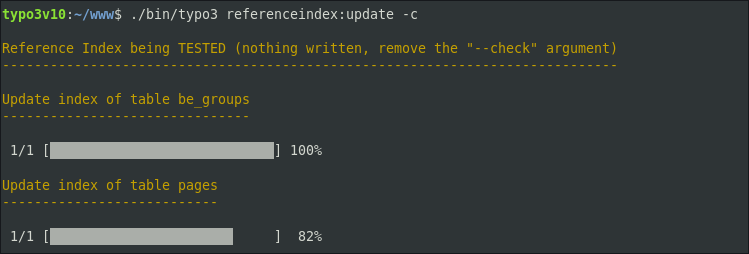
\includegraphics[width=0.85\linewidth]{ChangesForIntegrators/82062-ProgressForReferenceIndexUpdateOnCli.png}
	\end{figure}

\end{frame}

% ------------------------------------------------------------------------------
% Feature | 90425 | Add seo fields to info module

\begin{frame}[fragile]
	\frametitle{Modifiche per integratori}
	\framesubtitle{Modulo Info}

	\begin{itemize}
		\item I dettagli SEO e Social Media sono stati aggiunti al modulo Info:\newline
			\textbf{WEB} $\rightarrow$ \textbf{Info} $\rightarrow$ \textbf{Pagetree Overview}.
	\end{itemize}

	\begin{figure}
		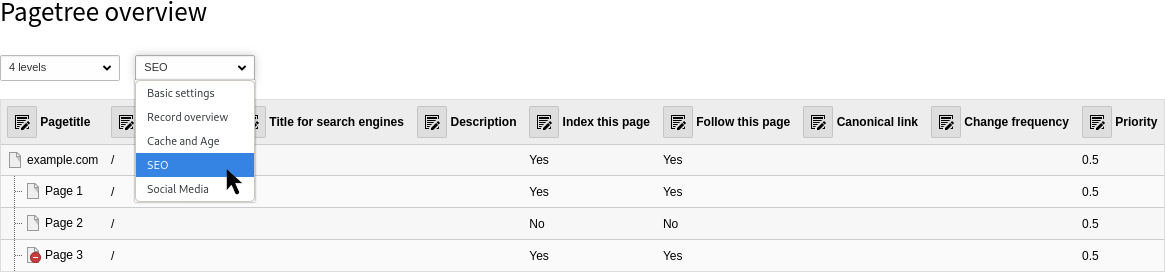
\includegraphics[width=0.85\linewidth]{ChangesForIntegrators/90425-AddSeoFieldsToInfoModule.png}
	\end{figure}

\end{frame}

% ------------------------------------------------------------------------------
% Feature | 59452 | scheduler:run command accepts multiple task options

\begin{frame}[fragile]
	\frametitle{Modifiche per integratori}
	\framesubtitle{Scheduler}

	% decrease font size for code listing
	\lstset{basicstyle=\tiny\ttfamily}

	\begin{itemize}
		\item È possibile eseguire più task quando si utilizza l'opzione \texttt{-}\texttt{-}\texttt{task}
	\end{itemize}

	\begin{figure}
		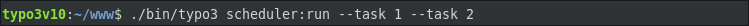
\includegraphics[width=0.85\linewidth]{ChangesForIntegrators/59452a-MultipleTasksInSchedulerCommand.png}
	\end{figure}

	\begin{itemize}
		\item L'output dettagliato può essere abilitato da \texttt{-}\texttt{v} e \texttt{-}\texttt{vv}
	\end{itemize}

	\begin{figure}
		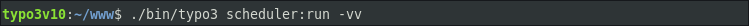
\includegraphics[width=0.85\linewidth]{ChangesForIntegrators/59452b-MultipleTasksInSchedulerCommand.png}
	\end{figure}

\end{frame}

% ------------------------------------------------------------------------------
% Feature | 90298 | Improve user info in BE User module

\begin{frame}[fragile]
	\frametitle{Modifiche per integratori}
	\framesubtitle{Moduli degli Utenti di Backend}

	\begin{itemize}
		\item Una nuova visualizzazione dettagliata dei record degli utenti backend mostra tutti i dati rilevanti.
		\item Ulteriori campi sono stati aggiunti alla funzione per confrontare gli utenti.
		\item Questa funzione ora tiene conto anche dei sottogruppi.
		\item L'interfaccia utente del modulo verrà ulteriormente modificata e ottimizzata.
		\item Queste modifiche rendono più semplice per gli integratori/amministratori controllare e confrontare
		    le autorizzazioni dell'utente senza diventare l'utente.
	\end{itemize}

\end{frame}

% ------------------------------------------------------------------------------
% Feature | 89894 | Separate system extensions from 3rd-party extensions visually

\begin{frame}[fragile]
	\frametitle{Modifiche per integratori}
	\framesubtitle{Extension Manager}

	Le estensioni di sistema e di terze parti ora possono essere elencate separatamente nell'Extension Manager.

	\begin{figure}
		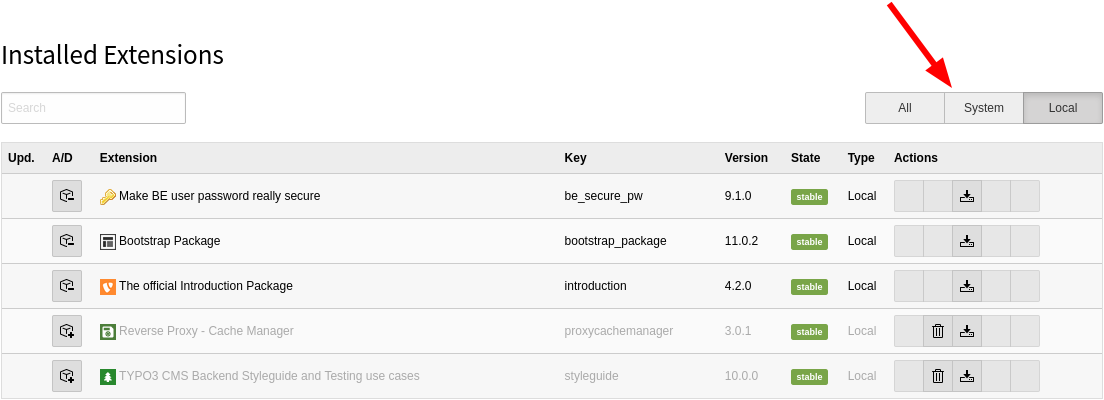
\includegraphics[width=0.9\linewidth]{BackendUserInterface/89894-SeparateSystemExtensionsFrom3rdPartyExtensionsVisually.png}
	\end{figure}

\end{frame}

% ------------------------------------------------------------------------------
% Feature | 90136 | Show application context in the Environment module

\begin{frame}[fragile]
	\frametitle{Modifiche per integratori}
	\framesubtitle{Environment Overview}

	L'attuale application context è ora mostrato nel modulo Environment:\newline
	\textbf{ADMIN TOOLS} $\rightarrow$ \textbf{Environment} $\rightarrow$ \textbf{Environment Overview}.

	\begin{figure}
		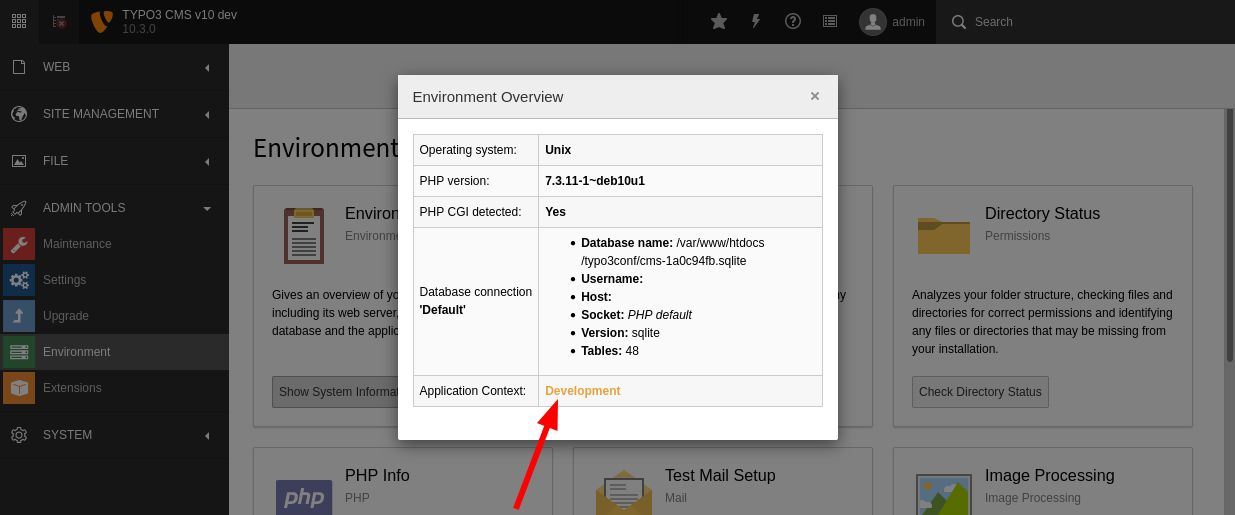
\includegraphics[width=0.9\linewidth]{ChangesForIntegrators/90136-ShowApplicationContextInTheEnvironmentModule.png}
	\end{figure}

\end{frame}

% ------------------------------------------------------------------------------
% Task | 89844 | Improve visual appearance of feature toggles

\begin{frame}[fragile]
	\frametitle{Modifiche per integratori}
	\framesubtitle{Funzione attiva/disattiva}

	L'aspetto grafico degli interruttori attiva/disattiva è stato migliorato:
	\newline\newline
	\smaller\textbf{TYPO3 < 10.3}\tabto{6cm}\textbf{TYPO3 >= 10.3}\normalsize

	\begin{figure}
		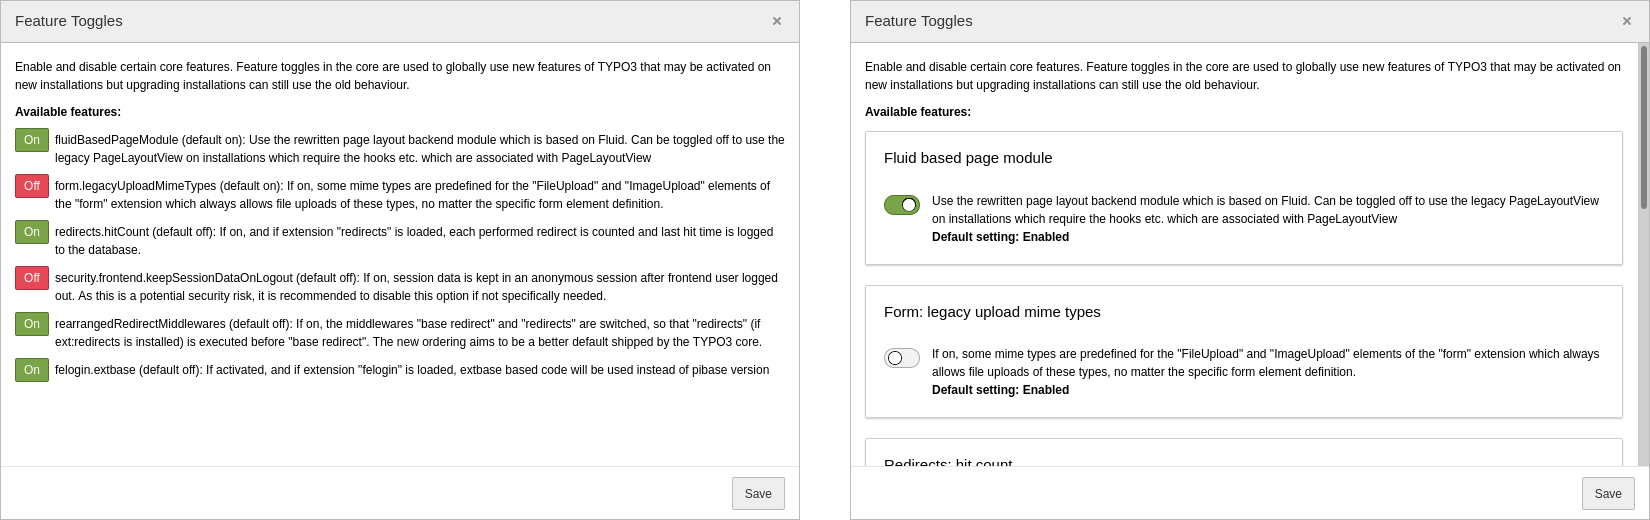
\includegraphics[width=1\linewidth]{ChangesForIntegrators/89844-ImproveVisualAppearanceOfFeatureToggles.png}
	\end{figure}

\end{frame}

% ------------------------------------------------------------------------------
% Feature | 89513 | Provide password recovery for backend users
%
%\begin{frame}[fragile]
%	\frametitle{Changes for Integrators}
%	\framesubtitle{Password Recovery Email}
%
%	\begin{itemize}
%
%		\item Password resets for backend users are only valid for 4 hours.\newline
%			This time limit is not configurable.
%		\item The function can optionally be disabled for all users or for admin users only to strengthen security.
%		\item If users share one email address, an alternative email text is used.
%		\item TCA field \texttt{be\_users.email} must not be set to \texttt{eval=email}.
%
%		\item The function only works for users, who:
%			\begin{itemize}
%				\item have an email address set,
%				\item have a password set, and
%				\item are not disabled/deleted.
%			\end{itemize}
%
%	\end{itemize}
%
%\end{frame}
%
% ------------------------------------------------------------------------------
